% -*- TeX-master: "main"; fill-column: 72 -*-

\section{Proposed syntax and semantics}
\label{syntax}

In this section, we define the syntax and semantics of the Arrays package for SBML Level~3 Version~1.  We describe the various data types and constructs defined in this package, then in \sect{examples}, we provide complete examples of using the constructs in example SBML models.

% -----------------------------------------------------------------------------
\subsection{Namespace URI and other declarations necessary for using this package}
\label{xml-namespace}

Every SBML Level~3 package is identified uniquely by an XML namespace URI.
For an SBML document to be able to use a given SBML Level~3 package, it
must declare the use of that package by referencing its URI.  The following
is the namespace URI for this version of the Arrays
package for SBML Level~3 Version~1:
\begin{center}
\uri{http://www.sbml.org/sbml/level3/version1/arrays/version1}
\end{center}

In addition, SBML documents using a given package must indicate whether
understanding the package is required for complete mathematical
interpretation of a model, or whether the package is optional.  This is
done using the attribute \token{required} on the \token{<sbml>} element in
the SBML document.  For the Arrays package, the value of
this attribute must be set to \val{true}.
The following fragment illustrates the beginning of a typical SBML model
using SBML Level~3 Version~1 and this version of the Arrays package:

\begin{example}
<?xml version="1.0" encoding="UTF-8"?>
<sbml xmlns="http://www.sbml.org/sbml/level3/version1/core" level="3" version="1"
      xmlns:fbc="http://www.sbml.org/sbml/level3/version1/arrays/version1" arrays:required="true">
\end{example}

\subsection{Primitive data types}

Section~3.1 of the \sbmlthreecore specification defines a number of primitive data types and also uses a number of XML Schema 1.0 data types~\citep{biron:2000}.  More specifically, we make use of \primtype{SId}, \primtype{string}, \primtype{int}, and \primtype{SIdRef}.  

% The Arrays package also defines two new primitive data types defined below.

%% QUESTION: IS THIS STILL NEEDED?  PERHAPS NOT FOR L3V2.

% \subsubsection{\emph{Type} \primtype{DimSId}}

% The type \primtype{DimSId} is derived from \primtype{SId} (SBML Level 3 Version 1 Core specification Section 3.1.7) and has identical syntax. The \primtype{DimSId} type is used as the data type for the identifiers of \Dimension objects. The purpose of having a separate type for such identifiers is to enable the space of possible dimension identifier values to be separated from the space of all other identifier values in SBML.  The scope of the \primtype{DimSId} is local to the enclosing object definition and is not visible outside the object definition.  The equality of \primtype{DimSId} values is determined by an exact character sequence match; i.e., comparisons of these identifiers must be performed in a case-sensitive manner.

%\subsubsection{\emph{Type} \{ 0, 1 \}}

%This type is simply the \primtype{int} type limited to the values of 0 and 1.

\subsection{Dimensions}
\label{sec:dimension}

As shown in \ref{fig:dimensions_uml}, the arrays package extends the \SBase class from core SBML with the addition of a list of \Dimension objects.  An object with a list of dimensions is an array, and the number of dimensions is equivalent to the number of \Dimension objects in the list.  Currently, SBML objects are restricted to at most three dimensions. 

\begin{figure}[tbhp]
  \centering
  % Requires \usepackage{graphicx}
  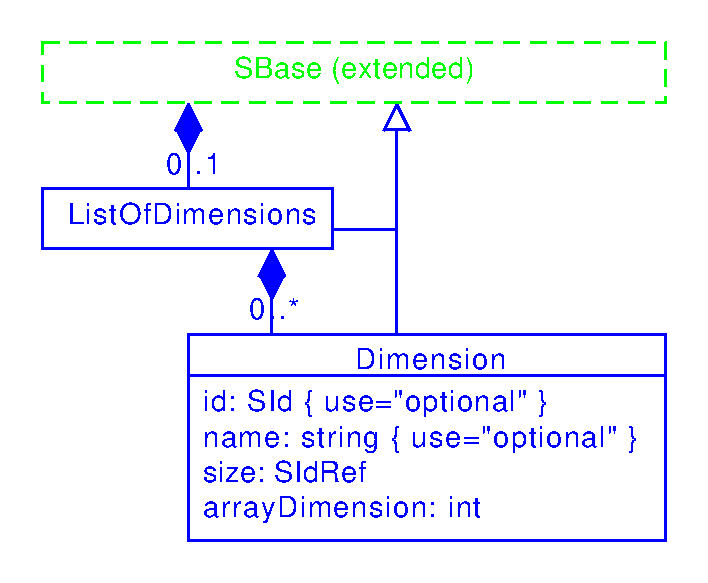
\includegraphics[width=0.5\textwidth]{images/dimensionsUML.pdf}\\
  \caption{A UML representation of the dimension classes. See \ref{conventions}} for conventions related to this figure. \label{fig:dimensions_uml}
\end{figure}

%\subsubsection{Dimension}

\paragraph{The \primtype{id} attribute}

The \Dimension object has an optional attribute, \primtype{id}, used to give the dimension an identifier.  The value of \primtype{id} must conform to the syntax permitted by the \primtype{SId} data type described in Section 3.1.7 of the SBML Level 3 Version 1 Core specification.  The scope of the \primtype{id} attribute is local to the enclosing object definition and is not visible outside the object definition.  The \primtype{id} attribute must be used as described in Section 3.3 of the SBML Level 3 Version 1 Core specification.  

\paragraph{The \primtype{name} attribute}

\Dimension also has an optional \primtype{name} attribute, of type \primtype{string} (see Section 3.1.1 and Section 3.3 of the SBML Level 3 Version 1 Core specification).  

\paragraph{The \primtype{size} attribute}

Each dimension of an array has a fixed size which is set with the \primtype{size} attribute.  The size attribute is of type \primtype{SIdRef} (see Section 3.1.8 of the SBML Level 3 Version 1 Core specification) and must refer to a \Parameter object instance defined in the model.  The \Parameter referenced must be \primtype{constant}, scalar, and have a defined initial value.

\paragraph{The \primtype{arrayDimension} attribute}

The \primtype{arrayDimension} attribute specifies which dimension is defined by this \Dimension object.  
Currently, the only allowed values for \primtype{arrayDimension} are 0, 1, and 2 (i.e., at most 3-dimensional arrays).  Also, there can be at most one \Dimension for each possible value of \primtype{arrayDimension}.  Finally, if a list of dimensions includes a \Dimension with \primtype{arrayDimension} value of 1, it must also include one with value 0.  Similarly, if it includes a \Dimension with \primtype{arrayDimension} value of 2, it must include ones with value 0 and 1, as well.  

\paragraph{Example}

As an example, a $10 \times 10$ array of compartments C could be defined as:

\begin{example}
<parameter id="n" value="10"/>
<compartment id="C" ...>
  <arrays:listOfDimensions>
    <arrays:dimension id="i" name="Row" size="n" arrayDimension="0"/>
    <arrays:dimension id="j" name="Column" size="n" arrayDimension="1"/>
  </arrays:listOfDimensions>
</compartment>
\end{example}

\paragraph{Dimension usage}

For SBML L3V1 core, only the following objects are allowed to be extended to include a list of dimensions:
\begin{itemize}
\item Parameters
\item Compartments
\item Species
\item Reactions
\item Species references
\item Rules
\item Initial assignments
\item Events
\item Event assignments
\item Constraints
\end{itemize}
Packages may choose to allow dimensions as desired.  For example, the hierarchical model composition package will allow dimensions on submodels.  

It is important to note that it is assumed that all elements of arrays created in this way share the same attribute values.  For example, if an initial value is specified for a compartment size, parameter value, or species amount then every element of the array takes that initial value.  To specify different initial values to different elements of an array, an initialAssignment should be used. 

\subsection{Indices}
\label{sec:index}

As shown in \ref{fig:indices_uml}, the arrays package extends the \SBase class from core SBML with the addition of a list of indices.  Each index in this list is used to specify an array index for a reference to an arrayed object specified in an attribute for this SBML element.    Each arrayed object specified in an attribute can have at most one index for each dimension specified for that object.  
For example, if the referenced object is a one-dimensional array, it can have one index.  If the referenced object is a two-dimensional array, it can have two indices.  In these cases, the referenced object is a scalar.  Note that if a two-dimensional array has only one index, the reference would return a one-dimensional array specified by this index.  If no index is specified, then the entire array is being referenced.  

\begin{figure}[tbhp]
  \centering
  % Requires \usepackage{graphicx}
  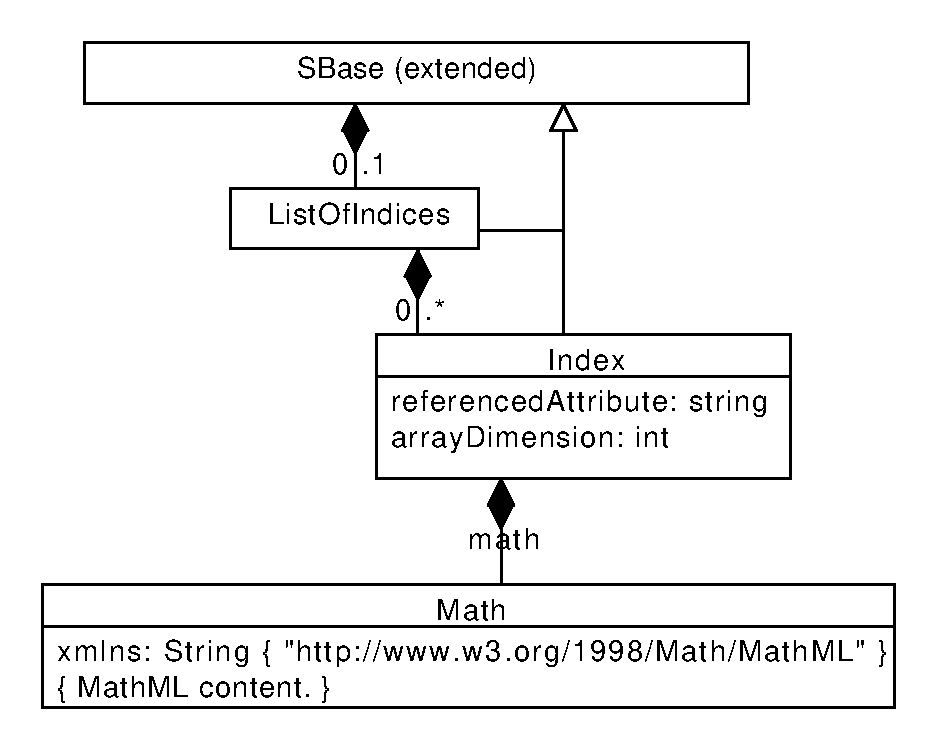
\includegraphics[width=0.65\textwidth]{images/indicesUML.pdf}\\
  \caption{A UML representation of the index classes. See \ref{conventions}} for conventions related to this figure. \label{fig:indices_uml}
\end{figure}

\paragraph{The \primtype{referencedAttribute} attribute}

The \primtype{referencedAttribute} attribute specifies the attribute of the SBML object to which this index is referencing.  

\paragraph{The \primtype{arrayDimension} attribute}

The \primtype{arrayDimension} attribute specifies which dimension this index corresponds to.
Currently, the only allowed values for \primtype{arrayDimension} are 0, 1, and 2 (i.e., at most 3-dimensional arrays can be indexed).  Also, there can be at most one \Index for each possible value of \primtype{arrayDimension}.  Finally, if a list of indices includes an \Index with \primtype{arrayDimension} value of 1, it must also include one with value 0.  Similarly, if it includes an \Index with \primtype{arrayDimension} value of 2, it must include ones with value 0 and 1, as well.

\paragraph{The \primtype{math} element}

The \primtype{math} element provides a mathematical expression which is evaluated to determine the index value for the reference.  Note that arrays are 0-based which means that an object of size $n$ can have index values between 0 and $n-1$.  When an index value computes to a value outside this range during simulation, this is an \emph{array out-of-bounds} error and simulation should terminate and report this error to the user.

\paragraph{Example}

The example below copies a reverse copy of the array in parameter x into parameter y.  

\begin{example}
<parameter id="n" value="10"/>
<parameter id="X" ...>
  <arrays:listOfDimensions>
    <arrays:dimension id="i" size="n" arrayDimension="0"/>
  </arrays:listOfDimensions>
</parameter>
<parameter id="Y" ...>
  <arrays:listOfDimensions>
    <arrays:dimension id="i" size="n" arrayDimension="0"/>
  </arrays:listOfDimensions>
</parameter>
<assignmentRule variable=Y>
  <arrays:listOfDimensions>
    <arrays:dimension id="i" size="n" arrayDimension="0"/>
  </arrays:listOfDimensions>
  <arrays:listOfIndices>
    <arrays:index referencedAttribute="variable" arrayDimension="0">
      <math>
        <apply>
          <minus/>
          <cn>9</cn>
          <ci>i</ci>
        </apply>
      </math>
    </arrays:index>
  </arrays:listOfIndices>
  <math>
    <apply>
      <selector/>
      <ci>X</ci>
      <ci>i</ci>
    </apply>
  </math> 
</assignmentRule>
\end{example}

Basically, this example is equivalent to:

\begin{example}
n = 10;
for (i=0; i < n; i++) {
    Y[9 - i] = X[i];
}
\end{example}

\paragraph{Index usage}

Only objects that have attributes of \primtype{SIdRef} type can have a list of indices.  For SBML L3V1 core, the following objects can have a list of indices:
\begin{itemize}
\item Model - conversionFactor
\item Species - compartment, conversionFactor
\item Reactions - compartment
\item Initial assignments - symbol
\item Rules - variable
\item Species references - species
\item Events assignments - variable
\end{itemize}
Similarly, for packages, any objects that have attributes of \primtype{SIdRef} type can also have indices.
In all cases, the object referenced by an index must, of course, be an arrayed object (i.e., have a specified dimension), and it must include the dimension being indexed.

Finally, the \primtype{math} element must be statically computable.  In other words, any identifier that appears in the math, other than a \Dimension \primtype{id} must be a constant.

\subsection{Mathematical formulas}

Section~3.4 of the \sbmlthreecore specification defines how mathematical expressions are expressed in SBML using a subset of MathML 2.0 \citep{w3c:2000b}.  In order to support arrays, the operators in this subset must be extended to support \token{ci} elements which are arrays.  For unary operators (the trigonometric operators, \token{abs}, \token{exp}, \token{ln}, \token{log}, \token{floor}, \token{ceiling}, \token{factorial}, and \token{not}), it is assumed that the operator is performed element-wise on each entry in the array.  For operators with two or more operands (the relational operators, \token{piecewise}, \token{plus}, \token{minus}, \token{times}, \token{divide}, \token{power}, \token{root}, \token{and}, \token{or}, and \token{xor}), it is again assumed that the operator is performed element-wise on each entry in the array.  In this case, it is required that each operand have the same dimensions with the same sizes or be a scalar value.  If an operand is a scalar value, it is assumed to be extended to an array of the same dimensions and sizes as the other operands, so it can be applied element-wise as well.  

The arrays package also extends the supported MathML subset to include the following:
\begin{itemize}
\item \emph{constructors}: \token{vector}
% {\bf matrix and matrixrow} 
\item \emph{element referenced operator}: \token{selector}
\item \emph{qualifier components}: \token{lowlimit}, \token{uplimit} \token{condition}
% \item \emph{linear algebra operators}: \token{vectorproduct}, \token{scalarproduct}, \token{outerproduct} 
%\begin{itemize}
%  \item{\bf determinant} %% Must be square matrix
%  \item {\bf transpose} %% Matrix
%  \item {\bf inverse} %% Matrix (?)
%\end{itemize}
%% Use lowlimit/uplimit 
\item \emph{sum product operators:} \token{sum}, \token{product}
%% Use condition to set range
\item \emph{quantifier operators:} \token{forall}, \token{exists}
\item \emph{statistics operators:} \token{mean}, \token{sdev}, \token{variance}, \token{median}, \token{mode}, \token{moment}, \token{momentabout}
\end{itemize}
